\documentclass[a4paper, 11pt]{article}
\usepackage[utf8]{inputenc}
\usepackage[swedish]{babel}
\usepackage{hyperref}
\usepackage{amsmath}
\usepackage[arrowdel]{physics}
\usepackage{bm}
\usepackage{graphicx}
\usepackage[margin=0.5in]{geometry}

\newcommand{\del}[2]{\partial_{#1}#2}
\newcommand{\inteval}[4]{\int\limits_{#1}^{#2}\dd{#3}#4}
\newcommand{\integ}[3]{\int\limits_{#1}\dd{#2}#3}
\newcommand{\cc}[1]{#1^{*}}
\newcommand{\leci}[1]{\varepsilon_{#1}}

\title{Sammanfattning av SH1014 Modern fysik}
\author{Yashar Honarmandi \\ yasharh@kth.se}
\date{\today}

\begin{document}

\maketitle

\begin{abstract}
	Detta ær en sammanfattning av kursen SH1014 Modern fysik.
\end{abstract}

\pagenumbering{roman}
\thispagestyle{empty}

\newpage

\tableofcontents

\newpage

\pagenumbering{arabic}

\section{Speciell relativitet}

\paragraph{Galileitransformationen}
Betrakta en statisk ram $S$ och en ram $S'$ som rör sig med konstant hastighet $\vb{u}$. Galileitransformen är den klassiska transformen av hastigheter och accelerationer mellan dessa system och ger
\begin{align*}
	\vb{r} = \vb{u}t + \vb{r}', \\
	\vb{v} = \vb{u} + \vb{v}', \\
	\vb{a} = \vb{a}'. \\
\end{align*}

\paragraph{Michelson-Morleys experiment}
Michelson-Morleys experiment visade att ljus omöjligt kunde propageras genom den postulerade etern.

Uppställningen som användes är (en mer avancerad variant av) Michelson-Morley-interferometern, som illustreras i figur \ref{fig:interferometer}.
\begin{figure}[!ht]
	\centering
	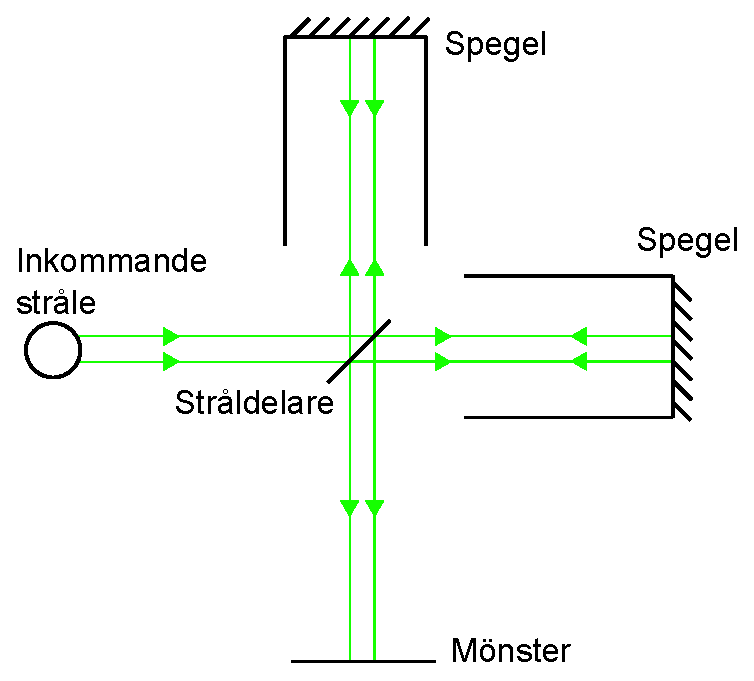
\includegraphics[width = 0.5\textwidth]{./Images/interferometer.eps}
	\caption{}
	\label{fig:interferometer}
\end{figure}

Ideen bakom experimentet var att de två "armarna" i uppställningen skulle röra sig med olika hastigheter relativt etern eftersom Jorden rör sig relativt Solen.

Om nu varje arm har längd $L$ och etern rör sig med en hastighet $u$ åt höger, tar ljuset tiden
\begin{align*}
	t_{\text{höger}} &= \frac{L}{c + u} + \frac{L}{c - u} \\
	                 &= L\frac{c - u + c + u}{c^{2} - u^{2}} \\
	                 &= \frac{2cL}{c^{2} - u^{2}} \\
	                 &= \frac{2L}{c}\frac{1}{1 - \frac{u^{2}}{c^{2}}}
\end{align*}
att röra sig till och från stråldelaren åt höger och tiden
\begin{align*}
	t_{\text{upp}} &= \frac{2L}{\sqrt{c^{2} - u^{2}}} \\
	               &= \frac{2L}{c}\frac{\sqrt{1 - \frac{u^{2}}{c^{2}}}}{1 - \frac{u^{2}}{c^{2}}},
\end{align*}
ty ljuset måste röra sig uppåt och motriktad hastigheten mot höger för att återvända till samma position i stråldelaren. Alltså borde skillnaden mellan tiden det tar för ljuset att röra sig de två vägarna ges av
\begin{align*}
	\Delta t = \frac{2L}{c}\frac{1 - \sqrt{1 - \frac{u^{2}}{c^{2}}}}{1 - \frac{u^{2}}{c^{2}}}.
\end{align*}
För Michelson och Morleys fal förutspådde de att de skulle se $0.4$ fransar i interferensmönstret, men de observerade $< 0.01$ fransar. Efter att ha upprepat sitt experiment ett halvår senare för att utesluta påverkan från Jordens position, konkluderade de med att det inte kunde finnas någon eter.

\paragraph{Einsteins postulat}
Baserad på Michelson-Morleys experiment, kom Einstein med följande postulat:
\begin{itemize}
	\item Fysikens lagar är de samma i alla inertialsystem.
	\item Ljushastigheten i vakuum har samma värde $c$ i alla inertialsystem.
\end{itemize}

\paragraph{Lorentztransformationen}
Lorentztransformationen är en transformation för att byta mellan olika referensramer. Den skiljer sig från Galileitransformationer, som inte är tillräcklig för att beskriva denna nya fysiken. Härledningen av denna kommer täckas här. Den är lite matematiskt involverad, så denna del av sammanfattningen är endast intressant för dig som tycker om sådant.

För att härleda Lorentztransformationen, betrakta två referensramar som sammanfallar vid $t = 0$ där den ena rör sig med en hastighet $v$ i $x$-riktning. För att beskriva transformationen, ansätter vi
\begin{align*}
	x' = k_{i}x_{i},
\end{align*}
där det summeras över alla rymdliga koordinater och tiden. Vi ansätter linjaritet eftersom det annars skulle kunna uppkomma accelererande rörelse i ett system utan att det är acceleration i ett annat, vilket skulle vara konstigt. Vidare antar vi att $x'$ ej beror av andra rymdliga kordinater, men att den kan bero av origos rörelse, och ansätter
\begin{align*}
	x' = k_{1}(x - vt).
\end{align*}
Antag nu att vi skickar ut en ljuspuls från origo vid $t = 0$. Vågfrontens avstånd från origo kommer beskrivas av
\begin{align*}
	x^{2} + y^{2} + z^{2} = c^{2}t^{2},
	x'^{2} + y^{2} + z^{2} = c^{2}t'^{2},
\end{align*}
eftersom ljuset skall ha samma fart i båda referensramer. Vi använder nu våran ansats för att transformera den andra ekvationen tillbaka, och får
\begin{align*}
	k_{1}^{2}x^{2} + y^{2} + z^{2} + k_{1}^{2}(v^{2}t^{2} - 2xvt) = c^{2}t'^{2}.
\end{align*}
Om vi sätter $t = t'$, får vi nu andra termer, och transformationen mislyckades. Vi åtgärder detta vid att ansätta
\begin{align*}
	t' = k_{t, 1}x + k_{t, 2}t.
\end{align*}
Detta ger
\begin{align*}
	k_{1}^{2}x^{2} + y^{2} + z^{2} + k_{1}^{2}(v^{2}t^{2} - 2xvt) = c^{2}(k_{t, 1}^{2}x^{2} + k_{t, 2}^{2}t^{2} + 2k_{t, 1}k_{t, 2}xt).
\end{align*}
För att transformationen skall lyckas, ger detta
\begin{align*}
	k_{1}^{2} - c^{2}k_{t, 1}^{2}      &= 1, \\
	vk_{1}^{2} + c^{2}k_{t, 1}k_{t, 2} &= 0, \\
	c^{2}k_{t, 2}^{2} - v^{2}k_{1}^{2} &= c^{2}.
\end{align*}
Vi kollar först fallet $v = 0$, motsvarande identitetstransformationen. Denna lösningen motsvarar $k_{1} = 1, k_{t, 1} = 0, k_{t, 2} = 1$, och en lösning för andra $v$ bör återskapa detta resultatet.

Vi inför nu
\begin{align*}
	\beta = \frac{v}{c}, \gamma = \frac{1}{\sqrt{1 - \beta^{2}}},
\end{align*}
och ekvationssystemet kan skrivas om till
\begin{align*}
	k_{1}^{2} - c^{2}k_{t, 1}^{2}       &= 1, \\
	\beta k_{1}^{2} + ck_{t, 1}k_{t, 2} &= 0, \\
	k_{t, 2}^{2} - \beta^{2}k_{1}^{2}   &= 1.
\end{align*}
Sista ekvationen kan skrivas som
\begin{align*}
	k_{1}^{2} = \frac{k_{t, 2}^{2} - 1}{\beta^{2}}.
\end{align*}
Den andra ekvationen kan skrivas som
\begin{align*}
	\frac{k_{t, 2}^{2} - 1}{\beta} + ck_{t, 1}k_{t, 2} = 0.
\end{align*}
Detta är en andragradsekvation i $k_{t, 2}$ med lösningar
\begin{align*}
	k_{t, 2} = \frac{-\beta ck_{t, 1} \pm\sqrt{\beta^{2}c^{2}k_{t, 1}^{2} + 4}}{2}.
\end{align*}
Vi kommer självklart se att transformationskoefficienterna är entydigt bestämda, men eftersom $k_{t, 1}$ fortfarande är okänd (basfallet ger inte ens tillräcklig information för att bestämma tecknet på den koeffeicienten) låter vi $\pm$-tecknet bli och fortsätter.

Vi får nu
\begin{align*}
	k_{1}^{2} &= \frac{\frac{\beta^{2}c^{2}k_{t, 1}^{2} + \beta^{2}c^{2}k_{t, 1}^{2} + 4 \mp 2\beta ck_{t, 1}\sqrt{\beta^{2}c^{2}k_{t, 1}^{2} + 4}}{4} - 1}{\beta^{2}} \\
	          &= \frac{2\beta^{2}c^{2}k_{t, 1}^{2} \mp 2\beta ck_{t, 1}\sqrt{\beta^{2}c^{2}k_{t, 1}^{2} + 4}}{4\beta^{2}} \\
	          &= \frac{\beta c^{2}k_{t, 1}^{2} \mp ck_{t, 1}\sqrt{\beta^{2}c^{2}k_{t, 1}^{2} + 4}}{2\beta}.
\end{align*}
Nu ser vi att valet av tecknet på $k_{t, 1}$ och valet av $\mp$ spelar roll - mer specifikt, om $k_{t, 1} > 0$ måste man välja $+$ och vice versa (annars skulle man få en imaginär transformationskoefficient, vilket skulle vara absurd när den beskriver en transformation mellan två observabler). Vi noterar att om den andra ekvationen skall uppfyllas, måste $k_{t, 1}k_{t, 2}$ vara negativ. Eftersom basfallet gav $k_{t, 2} = 1$, gissar vi att $k_{t, 1}$ är negativ (vadå, har du en bättre gissning?). Första ekvationen ger nu
\begin{align*}
	\frac{\beta c^{2}k_{t, 1}^{2} - ck_{t, 1}\sqrt{\beta^{2}c^{2}k_{t, 1}^{2} + 4}}{2\beta} - c^{2}k_{t, 1}^{2} = 1.
\end{align*}
Vi får rotuttrycket för sig själv och får
\begin{align*}
	-\frac{ck_{t, 1}}{2\beta}\sqrt{\beta^{2}c^{2}k_{t, 1}^{2} + 4} = 1 + \frac{1}{2}c^{2}k_{t, 1}^{2}.
\end{align*}
Vi har något positivt på båda sidor, och kan med ro i hjärtat kvadrera för att få
\begin{align*}
	\frac{c^{2}k_{t, 1}^{2}}{4\beta^{2}}(\beta^{2}c^{2}k_{t, 1}^{2} + 4) = 1 + c^{2}k_{t, 1}^{2} + \frac{1}{4}c^{4}k_{t, 1}^{4}.
\end{align*}
Gudarna är barmhärtiga, och detta förenklas till
\begin{align*}
	\left(\frac{1}{\beta^{2}} - 1\right)c^{2}k_{t, 1}^{2} &= 1, \\
	c^{2}k_{t, 1}^{2}                                     &= \frac{1}{\frac{1}{\beta^{2}} - 1} \\
	                                                      &= \frac{\beta^{2}}{1 - \beta^{2}}.
\end{align*}
Detta har (negativ) lösning
\begin{align*}
	k_{t, 1} = -\frac{\beta\gamma}{c}.
\end{align*}
Första ekvationen ger nu
\begin{align*}
	k_{1}^{2} &= 1 + c^{2}k_{t, 1}^{2} \\
	          &= 1 + \beta^{2}\gamma^{2} \\
	          &= \frac{1 - \beta^{2} + \beta^{2}}{1 - \beta^{2}} \\
	          &= \gamma^{2}.
\end{align*}
Vi ser att $\gamma$ har samma tecken för alla $\beta$, och eftersom vi sökte en positiv lösning för $\beta = 0$, väljer vi $k_{1} = \gamma$.

Sista ekvationen ger på helt samma sättet
\begin{align*}
	k_{1}^{2} = 1 + \beta^{2}k_{t, 2}^{2} = 1 + \beta^{2}\gamma^{2} = \gamma^{2},
\end{align*}
och med ett motsvarande argument får vi $k_{1} = \gamma$.

Om du är en matematiker, ser du kanske att ekvationerna vi utgick från är invarianta under teckenbyte av vissa koefficienter, och du kan komma fram till en lika bra lösning på dessa vid att byta tecken på några transformationskoefficienter. Dessa löser ekvationerna, men ger absolut inget samsvar med gammal och vältestad teori, vilket man typiskt inte vill att ens nya revolutionära teori skall göra.

Om du är en matematiker och ett petigt as, tycker du kanske att val av tecken kan bero av $\beta$. Det löser ju ekvationerna, trots allt. Detta är sant, men bara tanken på att förklara absurditeten i detta för dig gör ont. Om du tycker det är rimligt att göra så, kan du omöjligt ha smält konsekvenserna av dina tankar ordentligt. Jag skulle rekommendera dig att sätta dig med en kopp te och fundera både två och tre gånger över vad du föreslår. Nu är det sent, och jag vill lägga mig.

\subparagraph{Alternativ härledning}
Wow, dessa tar ju aldrig slut.

Vi kan i stället göra en härledning vid att låta Lorentztransformen vara linjär, och ställa följande krav på den:
\begin{itemize}
	\item Ljusets hastighet är den samma i båda referensramer, dvs. att $x = ct$ och $x' = ct'$ måste gälla samtidigt.
	\item Den inversa transformen måste motsvara transformen när hastigheten $v$ till den rörliga referensramen byter tecken.
\end{itemize}
Vi skriver Lorentztransformen som
\begin{align*}
	x' = Ax + Bt, \\
	t' = Cx + Dt.
\end{align*}
Om man betraktar punkten $x' = 0$, har denna uppenbarligen rörelse $x = vt$, vilket implicerar $\frac{B}{A} = -v$. Lorentztransformen kan då skrivas som
\begin{align*}
	x' = A(x - vt).
\end{align*}
Kravet som rör att ljushastigheten är konstant ger
\begin{align*}
	ct' &= A(c - v)t, \\
	ct  &= A(c + v)t'
\end{align*}
för transformen och den inversa transformen av $x'$. Produkten av dessa två ekvationerna är
\begin{align*}
	c^{2}tt' = A^{2}(c^{2} - v^{2})tt',
\end{align*}
vilket implicerar
\begin{align*}
	A^{2}  = \gamma^{2}.
\end{align*}
Återigen skulle man kunna leka med tecknet, men vi bara väljer en positiv konstant och låter det bli med det.

För att bestämma transformationskoefficienterna för tid, försöker vi att Lorentztransformera den inversa transformen. Den inversa transformen ges av
\begin{align*}
	x = \gamma(x' + vt'),
\end{align*}
och transformation av denna ger
\begin{align*}
	x = \gamma(x' + vCx + vDt).
\end{align*}
Vi löser denna för $x'$ och får
\begin{align*}
	x' = \left(\frac{1}{\gamma} - vC\right)x - vDt.
\end{align*}
Om detta skall motsvara den ursprungliga transformen, måste
\begin{align*}
	\frac{1}{\gamma} - vC &= \gamma, \\
	-vD                   &= -v\gamma.
\end{align*}
Detta har lösningar
\begin{align*}
	D &= \gamma, \\
	C &= \frac{1}{v}\frac{1 - \gamma^{2}}{\gamma} \\
	  &= \frac{1}{v}\frac{1 - \frac{1}{1 - \beta^{2}}}{\gamma} \\
	  &= -\frac{1}{v}\frac{\frac{\beta^{2}}{1 - \beta^{2}}}{\gamma} \\
	  &= -\frac{\beta}{c}\frac{\gamma^{2}}{\gamma} \\
	  &= -\frac{\beta\gamma}{c}.
\end{align*}

\paragraph{Formler för Lorentztransformationen}
Lorentztransformationen ges av
\begin{align*}
	x' = \gamma(x - vt), t' = \gamma\left(t - \frac{\beta}{c}x\right),
\end{align*}
med
\begin{align*}
	\beta = \frac{v}{c}, \gamma = \frac{1}{\sqrt{1 - \beta^{2}}}.
\end{align*}
Den inversa Lorentztransformationen fås vid att lösa ut ekvationerna för $x$ och $t$, och ges av
\begin{align*}
	x = \gamma(x' + vt'), t = \gamma\left(t' + \frac{\beta}{c}x'\right).
\end{align*}
Med de givna skalfaktorerna ser vi att för små hastigheter går detta över i Galileitransformer, medan inga hastigheter över $c$ tillåts.

\paragraph{Samtidighet}
Betrakta två händelser som inträffer med en tidsskillnad $\Delta t$ mätt i inertialramen. Lorentztransformationen ger
\begin{align*}
	\Delta t = \gamma(\Delta t' + \frac{\beta}{c}\Delta x').
\end{align*}
Detta implicerar att även om händelserna är samtidiga i en referensram, är de inte nödvändigtvis det i den andra. Om tidsskillnaden mäts i den rörliga ramen, kan den skrivas som
\begin{align*}
	\Delta t' = \gamma(\Delta t - \frac{\beta}{c}\Delta x).
\end{align*}

\paragraph{Tidsdilation}
Betrakta två händelser som inträffer vid samma position i den rörliga ramen. Lorentztransformationen ger
\begin{align*}
	\Delta t = \gamma\Delta t',
\end{align*}
och det mäts en längre tidsskilland mellan händelserna i den statiska ramen. Symmetrierna i ekvationen ovan ger att om händelserna inträffer vid samma position i den statiska ramen, observeras tidsdilatation i den rörliga ramen.

Med andra ord: Observatörer som ej är statiska relativt två händelser mäter en längre tidsskillnad mellan händelserna än observatörer som är statiska relativt händelsen.

\paragraph{Längdkontraktion}
Lorentztransformationen av avståndet mellan två händelser ges av
\begin{align*}
	\Delta x' &= \gamma(\Delta x - v\Delta t), \\
	\Delta x  &= \gamma(\Delta x' + v\Delta t')
\end{align*}
Betrakta två händelser som rör sig med den rörliga ramen och inträffer vid samma tidspunkt i den rörliga ramen. Lorentztransformationen ger
\begin{align*}
	\Delta x = \frac{1}{\gamma}\Delta x',
\end{align*}
och det mäts ett kortare avstånd mellan händelserna i inertialramen. Symmetrien ger ett motsvarande resultat om händelserna är samtidiga i den statiska ramen.

Med andra ord: Observatörer som ej är statiska relativt två händelser mäter ett kortare avstånd mellan händelserna än observatörer som är statiska relativt händelsen.

\paragraph{Tvillingparadoxen}
Betrakta två tvillingar, där tvilling $A$ stannar på Jorden hela sitt liv och tvilling $B$ reser till en planet långt borta och tillbaka med en relativistisk hastighet. $A$ får att hen har åldrats mer än sin tvilling eftersom denna har upplevd tidsdilatation. Men $B$ upplever att hen är statisk och att $A$ rör sig. Därmed upplever $A$ tidsdilatation enligt $B$, och $B$ åldrats mer. Hur kan båda tycka att de är äldst när $B$ kommer tillbaka?

För att lösa paradoxen, antag att $A$ och $B$ skickar ut ljuspulser med något fast tidsintervall för att hålla koll på hur gamla varandra är. Eftersom ljuset har samma hastighet i alla inertialramer, måste antal pulser vara ett mått på ålder som både $A$ och $B$ kan enas om.

Låt planeten vara ett avstånd $x = cT$ från Jorden, och låt $B$ röra sig med en hastighet $v = \beta c$ mot antingen planeten eller Jorden. Enligt $A$ tar det $t = \frac{T}{\beta}$ att nå planeten, och $t = \frac{2T}{\beta}$ att åka fram och tillbaka. $B$s position ges då enligt $A$ av
\begin{align*}
	s =
	\begin{cases}
		\beta ct,       &t < \frac{T}{\beta}, \\
		c(2T - \beta t), &\frac{T}{\beta} < t < \frac{2T}{\beta}.
	\end{cases}
\end{align*}
Om varje tvilling skickar ut en ljuspuls med tidsintervall $\Delta t$, mottar $B$ ljuspuls nummer $n$ enligt $A$ när
\begin{align*}
	c(t_{B, n} - n\Delta t) = s(t_{B, n}).
\end{align*}
Vi betraktar först ljuspulser som mottas när $B$ är på väg mot planeten. Dessa mottas vid tid
\begin{align*}
	t_{B, n} = \frac{n}{1 - \beta}\Delta t. 
\end{align*}
$A$ mottar ljuspulser som skickas ut med tidsintervall $\gamma\Delta t$ och ljuspuls nummer $n$ mottas när
\begin{align*}
	s(\gamma n\Delta t) - c(t_{A, n} - \gamma n\Delta t) = 0.
\end{align*}
Vi betraktar igen ljuspulser som mottas när $B$ är på väg mot planeten. Dessa mottas vid tid
\begin{align*}
	c\beta\gamma n\Delta t - c(t_{A, n} - \gamma n\Delta t) = 0, \\
	t_{A, n} = (1 + \beta)\gamma n\Delta t.
\end{align*}

Vi betraktar vidare ljuspulser som mottas av $B$ på väg mot Jorden. Dessa mottas när
\begin{align*}
	c(t_{B, n} - n\Delta t) &= c(2T - \beta t_{B, n}), \\
	t_{B, n}                &= \frac{2T + n\Delta t}{1 + \beta}.
\end{align*}
$A$ mottar ljuspuls nummer $n$ när
\begin{align*}
	c(2T - \beta\gamma n\Delta t) - c(t_{A, n} - \gamma n\Delta t) &= 0, \\
	t_{A, n}                                                        &= 2T + (1 - \beta)\gamma n\Delta t.
\end{align*}

Skillnaden mellan de två kommer från att $B$ mottar sin sista puls på väg mot planeten vid $t = \frac{T}{\beta}$, medan $A$ mottar sista pulsen från färden till planeten vid tiden
\begin{align*}
	t = \frac{1 + \beta}{\beta}T.
\end{align*}
Pulserna från de olika etapperna når $A$ och $B$ med olika tidsintervall. Eftersom ændringen i tidsintervall inträder tidigare för $B$ än $A$, och detta kommer ge att de är överens om hur gamla de är.

För att kunna jämföra åldern, vill vi nu veta hur många pulser varje tvilling mottar under de två etapperna. Under resan till planeten mottar $B$
\begin{align*}
	n_{A\to B} = \frac{T}{\Delta t}\frac{1 - \beta}{\beta}
\end{align*}
pulser, medan $B$ har skickat ut
\begin{align*}
	n_{B} = \frac{T}{\beta\gamma\Delta t}
\end{align*}
pulser. Under resan tillbaka till Jorden mottar $B$
\begin{align*}
	n_{A\to B} = 2T\frac{1}{\beta\Delta t} - \frac{T}{\Delta t}\frac{1 - \beta}{\beta} = \frac{T}{\beta\Delta T}(2 - 1 + \beta) = \frac{T(1 + \beta)}{\beta\Delta t}
\end{align*}
pulser, medan $B$ har skickat ut
\begin{align*}
	n_{B} = \frac{T}{\beta\gamma\Delta t}
\end{align*}
pulser. Alltså upplever $B$ att den åldras långsammare med en faktor
\begin{align*}
	\frac{n_{A\to B}}{n_{B}} = \frac{\frac{T}{\Delta t}\frac{1 - \beta}{\beta}}{\frac{T}{\beta\gamma\Delta t}} = (1 - \beta)\gamma
\end{align*}
under resan till planeten, dvs. under tiden $\frac{T}{\beta\gamma}$ och snabbare med en faktor
\begin{align*}
	\frac{n_{A\to B}}{n_{B}} = \frac{\frac{T(1 + \beta)}{\beta\Delta t}}{\frac{T}{\beta\gamma\Delta t}} = (1 + \beta)\gamma
\end{align*}
under den resterande tiden. Alltså är det slutliga förhållandet i ålder
\begin{align*}
	\frac{(1 - \beta)\frac{T}{\beta} + (1 + \beta)\frac{T}{\beta}}{2\frac{T}{\gamma\beta}} = \frac{1 - \beta + 1 + \beta}{2}\gamma = \gamma.
\end{align*}

På andra sidan mottar $A$
\begin{align*}
	n_{B\to A} = \frac{T}{\gamma\beta\Delta t}
\end{align*}
pulser som skickades från färden till planeten under tiden $\frac{1 + \beta}{\beta}T$, medan $A$ har skickat ut
\begin{align*}
	n_{A} = \frac{1 + \beta}{\beta}\frac{T}{\Delta t}
\end{align*}
pulser under samma tiden. $A$ mottar även
\begin{align*}
	n_{B\to A} = \frac{2T}{\gamma\beta\Delta t} - \frac{T}{\gamma\beta\Delta t} = \frac{T}{\gamma\beta\Delta t}
\end{align*}
pulser från färden tillbaka till Jorden, medan $A$ har skickat ut
\begin{align*}
	n_{A} = \frac{\frac{2T}{\beta} - \frac{1 + \beta}{\beta}T}{\Delta t} = \frac{2T - (1 + \beta)T}{\beta\Delta t} = \frac{T(1 - \beta)}{\beta\Delta t}
\end{align*}
pulser under den återstående tiden. Alltså upplever $A$ att den äldas snabbare med en faktor
\begin{align*}
	\frac{n_{B\to A}}{n_{A}} = \frac{\frac{T}{\gamma\beta\Delta t}}{\frac{1 + \beta}{\beta}\frac{T}{\Delta t}} = \frac{1}{(1 + \beta)\gamma}
\end{align*}
när den får signaler från resan till planeten och långsammare med en faktor
\begin{align*}
	\frac{n_{B\to A}}{n_{A}} = \frac{\frac{T}{\gamma\beta\Delta t}}{\frac{T(1 - \beta)}{\beta\Delta t}} = \frac{1}{(1 - \beta)\gamma}
\end{align*}
när den får signaler från resan till Jorden. Det slutliga förhållandet i ålder blir då
\begin{align*}
	\frac{\frac{1}{(1 + \beta)\gamma}\frac{1 + \beta}{\beta}T + \frac{1}{(1 - \beta)\gamma}(\frac{2T}{\beta} - \frac{1 + \beta}{\beta}T)}{\frac{2T}{\beta}} = \frac{1 + \frac{1 - \beta}{1 - \beta}}{2}\frac{1}{\gamma} = \frac{1}{\gamma},
\end{align*}
och de två är överens om att tvillingen på Jorden åldras snabbast.

\paragraph{Relativistisk Dopplereffekt}
Betrakta återigen två olika system, där det rörliga systemet rör sig med en vinkel $\theta$ från linjen mellan $O$ och $O'$, som är parallell med $x$-axeln. Från $O'$ skickas det ut ljuspulser vid $t_{1}'$ och $t_{2}'$. Lorentztransformationerna ger att ljuset skickas ut vid tider
\begin{align*}
	t_{1} = \gamma t_{1}', \\
	t_{2} = \gamma t_{2}'.
\end{align*}
Om första pulsen skickas ut vid avstånd $x_{1}$, skickas den andra ut vid avstånd
\begin{align*}
	x_{2} = x_{1} + \gamma v(t_{2}' - t_{1}')\cos{\theta},
\end{align*}
där vi har approximerat att avståndet $S'$ rör sig normalt på $x$-axeln är litet. Ljuspulserna når därmed origo vid tid
\begin{align*}
	t_{O1} &= t_{1} + \frac{x_{1}}{c}, \\
	t_{O2} &= t_{2} + \frac{x_{2}}{c} \\
	       &= t_{2} + \frac{x_{1} + \gamma v(t_{2}' - t_{1}')\cos{\theta}}{c} \\
	       &= \frac{x_{1}}{c} + \gamma t_{2}'(1 + \beta\cos{\theta}) - \gamma t_{1}'\beta\cos{\theta}.
\end{align*}
Vi inför periodtiden $\Delta t' = t_{2}' - t_{1}'$, och får
\begin{align*}
	\Delta t_{O} &= \gamma t_{2}'(1 + \beta\cos{\theta}) - \gamma t_{1}'(1 + \beta\cos{\theta}) \\
	             &= \gamma (1 + \beta\cos{\theta})\Delta t'.
\end{align*}
Frekvensen för ljuspulsen ges då av
\begin{align*}
	f_{\text{obs}} = \frac{1}{\gamma(1 + \beta\cos{\theta})}f_{\text{källa}}.
\end{align*}

\paragraph{Lorentztransformation av hastigheter}
Vi använder differentialerna
\begin{align*}
	\dd{x} = \gamma(\dd{x'} + v\dd{t'}), \\
	\dd{t} = \gamma(\dd{t'} + \frac{\beta}{c}\dd{x'})
\end{align*}
och får hastigheterna
\begin{align*}
	u_{x} &= \dv{x}{t} = \frac{\dd{x'} + v\dd{t'}}{\dd{t'} + \frac{\beta}{c}\dd{x'}} = \frac{u_{x}' + v}{1 + \frac{\beta}{c}u_{x}'}, \\
	u_{y} &= \frac{u_{y}'}{1 + \frac{\beta}{c}u_{x}'}, \\
	u_{z} &= \frac{u_{z}'}{1 + \frac{\beta}{c}u_{x}'}.
\end{align*}

\paragraph{Relativistisk rörelsemängd}
Betrakta studsen som illustreras i figur \ref{fig:collision_inertial}.
\begin{figure}[!ht]
	\centering
	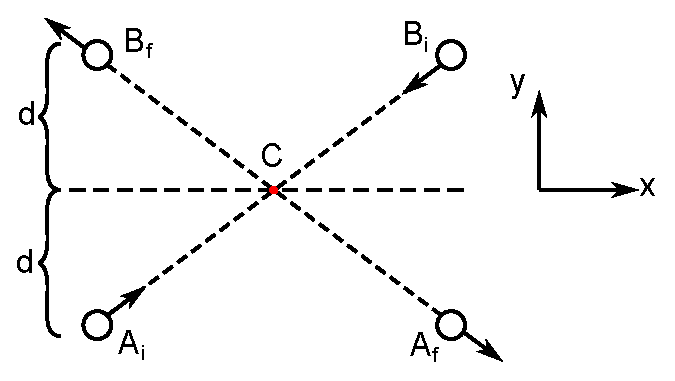
\includegraphics[width = 0.5\textwidth]{./Images/collision_inertial.eps}
	\caption{Illustration}
	\label{fig:collision_inertial}
\end{figure}

Vi antar här att rörelsen kan vara relativistisk i $x$, men approximeras som klassisk i $y$. Om partiklerna har samma massa (och hastighet), är masscentrum statiskt i $C$. Studsen är vidare symmetrisk kring masscentrum, och därmed måste både $A$ och $B$ ha samma hastighet i $x$-riktning.

Vi kan alternativt betrakta studsen i en referensram som följer partikeln $A$ i $x$-riktning, vilket illustreras i figur \ref{fig:collision_following}.
\begin{figure}[!ht]
	\centering
	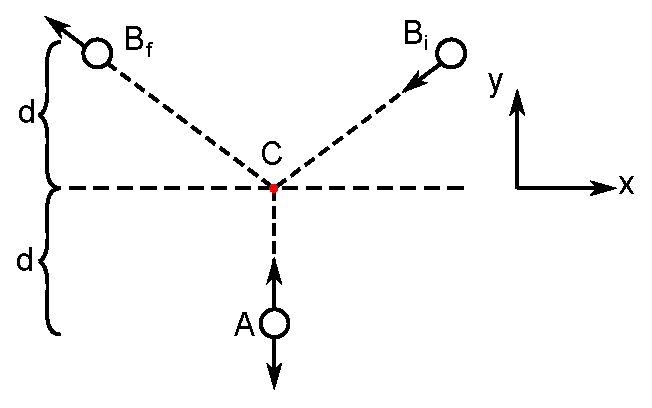
\includegraphics[width = 0.5\textwidth]{./Images/collision_following.eps}
	\caption{Illustration}
	\label{fig:collision_following}
\end{figure}
Symmetriargumentet gäller även här.

Båda system är inertialsystem, och därmed är rörelsesmängden bevarad i båda system.

Vi definierar tiden $t_{0}$ som det tar för $A$ att röra sig avståndet $d$ upp och ned i $A$:s referensram. Ändringen i rörelsemängd ges då av
\begin{align*}
	\Delta p_{A, y} = -2m_{A}\frac{d}{t_{0}} - 2m_{A}\frac{d}{t_{0}} = -4m_{A}\frac{d}{t_{0}}, \\
	\Delta p_{B, y} = 2m_{B}\frac{d}{t} + 2m_{B}\frac{d}{t} = 4m_{B}\frac{d}{t},
\end{align*}
där tiden $t$ är tiden det tar för $B$ att röra sig upp och ned i denna referensramen. Eftersom rörelsen i $y$-riktning är klassisk, är denna tiden $t_{0}$ i en referensram som följer $B$ på samma sättet. Vi transformerar därmed från ramen som följer $A$ till ramen som följer $B$. Om ramen som följer $A$ rör sig med en hastighet $v$ relativt ramen som följer $B$, får man efter transformation att
\begin{align*}
	\Delta p_{B, y} = 4m_{B}\frac{d}{\gamma t_{0}}.
\end{align*}
Den totala ändringen i rörelsemängdsmoment är lika med $0$, vilket ger
\begin{align*}
	m_{B} = \gamma m_{A}.
\end{align*}
Eftersom rörelsen i $y$-riktning är klassisk, kan $A$:s massa nu ersättas av vilomassan $m_{0}$, som är $A$:s massa mätt i sitt eget inertialsystem. Eftersom de två har samma vilomassa, ger detta
\begin{align*}
	m = \gamma m_{0}.
\end{align*}
Den relativistiska rörelsemängden ges därmed av
\begin{align*}
	p = mv = \gamma m_{0}v.
\end{align*}

\paragraph{Relativistisk energi}
Newtons andra lag ger
\begin{align*}
	F = \dv{t}\left(mv\right).
\end{align*}
Om kraftsumman $F$ får verka på en partikel som börjar från vilo, ges dens kinetiska energi av
\begin{align*}
	T = \int F\cdot\dd{s} = \int\dv{t}\left(mv\right)\cdot v\dd{t} = \int v\cdot\dd{(mv)} = \int v^{2}\dd{m} + mv\cdot\dd{v}.
\end{align*}
Lorentztransformationen av massa ger
\begin{align*}
	m^{2}\gamma^{2} = m_{0}^{2},\ m^{2}(c^{2} - v^{2}) = m_{0}^{2}c^{2}.
\end{align*}
Vid att beröäkna differentialen av båda sidor får
\begin{align*}
	2mc^{2}\dd{m} - 2mv^{2}\dd{m} - 2m^{2}v\cdot\dd{v} = 0, c^{2}m = v^{2}\dd{m} + mv\cdot\dd{v},
\end{align*}
vilket insatt i integralen ger
\begin{align*}
	T = \int c^{2}\dd{m} = c^{2}(m - m_{0}) = m_{0}c^{2}(\gamma - 1).
\end{align*}
Detta kan alternativt skrivas som
\begin{align*}
	mc^{2} = T + m_{0}c^{2},
\end{align*}
vilket tolkades som ett uttryck för totala energin som innehåller en konstant viloenergi $m_{0}c^{2}$ (obs: Ej en potentiell energi!). Därmed ges den totala energin av
\begin{align*}
	E = mc^{2} = T + m_{0}c^{2}.
\end{align*}

\paragraph{Relation mellan energi och rörelsemängd}
Vi har nu fått
\begin{align*}
	p^{2} = \gamma^{2}m_{0}^{2}v^{2}, E^{2} = \gamma^{2}m_{0}^{2}c^{4}.
\end{align*}
Energin i kvadrat kan skrivas som
\begin{align*}
	E^{2} = \gamma^{2}m_{0}^{2}c^{4} = \gamma^{2}m_{0}^{2}c^{4}\left(\frac{1}{\gamma^{2}} + \beta^{2}\right),
\end{align*}
eftersom $\gamma = \frac{1}{\sqrt{1 - \beta^{2}}}$. Vi får vidare
\begin{align*}
	E^{2} &= m_{0}^{2}c^{4} + m_{0}^{2}v^{2}c^{2} \\
	      &= m_{0}^{2}c^{4} + p^{2}c^{2}.
\end{align*}

\section{Allmän relativitetsteori}

\paragraph{Gravitationell tidsdilatation}
Betrakta två observatorer i ett tyngdfält med (svag) uniform fältstyrka $g$ som befinner sig på olika positioner med en höjdskillnad $h$. Då upplever observatören högre upp i fältet en tidsdilatation
\begin{align*}
	\Delta t' = (1 + \frac{gh}{c^{2}})\Delta t.
\end{align*}
Om man har ett icke-uniformt tyngdfält, kan man i stället använda att för små $\Delta h$ gäller att
\begin{align*}
	\frac{\Delta t(h + \Delta{h})}{\Delta t(h)}       &= (1 + \frac{g(h)}{c^{2}}\Delta{h}), \\
	\prod\frac{\Delta t(h_{i})}{\Delta t(h_{i - 1})}  &= \frac{\Delta t(h)}{\Delta t(h_{0})} &= (1 + \sum\Delta{h}\frac{g(h_{i})}{c^{2}})
\end{align*}
med $h_{i} = h_{0} + i\Delta{h}$, och i gränsen $\Delta h\to 0$
\begin{align*}
	\frac{\Delta t(h)}{\Delta t(h_{0})} = 1 + \inteval{h_{0}}{h}{x}{\frac{g(x)}{c^{2}}}.
\end{align*}

\section{Kvantmekanik}

\paragraph{Brister i klassisk fysik}
Redan innan kvantmekaniken formulerades, fanns det brister i det experimentella beviset för den klassiska fysiken.

\subparagraph{Ultravioletta katastrofen}
Ett bevis var att den klassiska förutsägelsen av svartkroppsstrålning var
\begin{align*}
	I(\nu, T) = \frac{2kT\nu^{2}}{c^{2}},
\end{align*}
som divergerar för stora frekvenser. Observationer av svartkroppsstrålning var naturligtvis inte i närheten av detta utan gick mot $0$ även för höga frekvenser.

Max Planck sägs att ha upptäckt kvantmekaniken vid att härleda intensitetsfördelningen för svartkroppsstrålning under antagandet att energinivåerna i kroppen var diskreta kvanta av $h\nu$, där $h$ är den nu införda Plancks konstant. Han fick
\begin{align*}
	I(\nu, T) = \frac{2h\nu^{3}}{c^{2}}\frac{1}{e^{\frac{h\nu}{kT}} - 1}.
\end{align*}
Denna går både mot $0$ för höga frekvenser och beter sig som den klassiska förutsägelsen vid  låga frekvenser. Einstein gissade senare att $h\nu$ var energien för partiklarna som bygger upp ljus - fotoner.

\subparagraph{Fotoelektriska effekten}
Om man bestrålar metaller med elektromagnetisk strålning, frigörs elektroner (upptäckta vid det här laget) från metallet. Man kunne sätta metallet i närheten av en anod så att en spänningsskillnad mellan metallet och anoden kunde attrahera metaller till anoden. Vid at elektriskt koppla de två samman, kunde man mäta strömmen som orsakades av de frigjorda elektronerna. Det som observerades var:
\begin{itemize}
	\item Det frigjordes bara elektroner om den inkommande strålningen hade en frekvens över en viss gränsfrekvens.
	\item Under denna gränsfrekvensen spelade strålningsintensiteten ingen roll.
	\item Över gränsfrekvensen mättes den maximala elektronenergin som $E = h\nu - W$.
\end{itemize}

Detta var svårt att förklara med klassisk fysik.

\subparagraph{Comptonspridning}
Elektromagnetisk strålning kan spridas på elektroner. Klassiskt är det svårt att förklara spridningsmönstret som uppstår, eftersom elektromagnetisk strålning är vågor. Däremot kan man anta att strålningen består av fotoner med rörelsemängd och energi enligt speciell relativitetsteori och resultaten från fotoelektriska effekten, som illustrerad i figur \ref{fig:compton_collision}.

\begin{figure}[!ht]
	\centering
	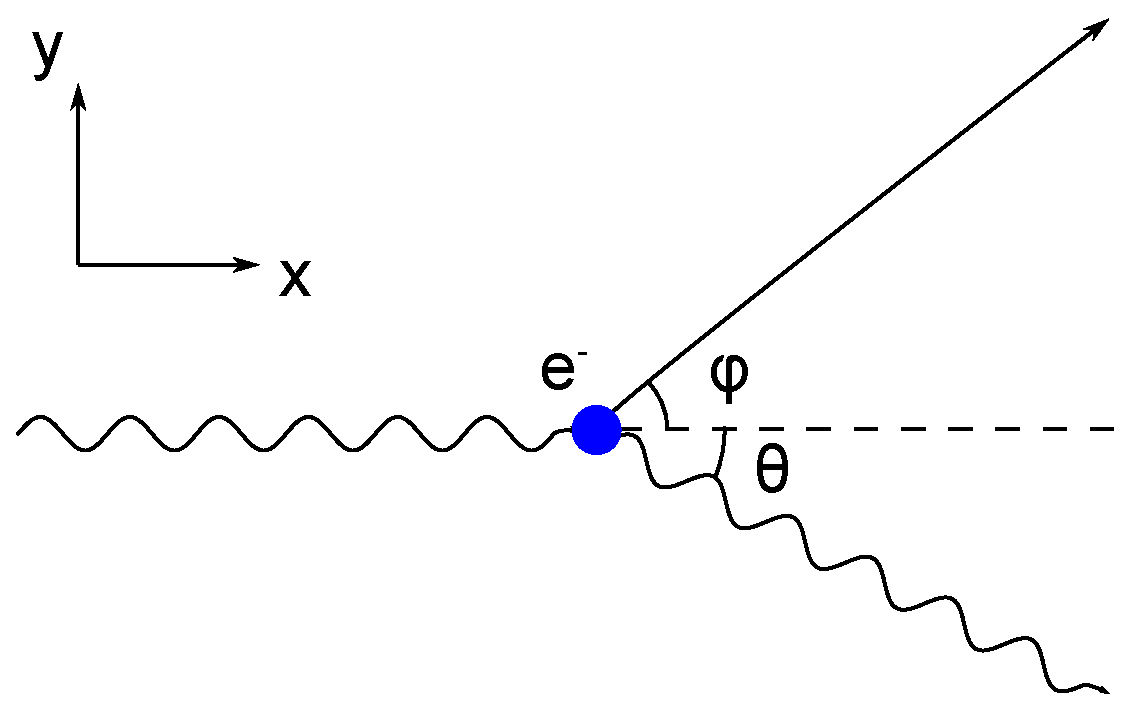
\includegraphics[width = 0.5\textwidth]{./Images/compton_collision.eps}
	\caption{Illustration av studs mellan en foton och en elektron.}
	\label{fig:compton_collision}
\end{figure}

Energins bevarande ger
\begin{align*}
	h\nu + m_{e, 0}c^{2} = E_{e} + h\nu'
\end{align*}
och rörelsemängdens bevarande ger
\begin{align*}
	h\frac{\nu}{c} = h\frac{\nu'}{c}\cos{\phi} + p_{e}'\cos{\theta}, \\
	h\frac{\nu'}{c}\sin{\phi} - p_{e}'\sin{\theta} = 0.
\end{align*}
Vi omformulerar förste rörelsemängdekvationen till
\begin{align*}
	h\frac{\nu}{c} - h\frac{\nu'}{c}\cos{\phi} = p_{e}'\cos{\theta}
\end{align*}
och kvadrerar för att få
\begin{align*}
	h^{2}\frac{\nu^{2}}{c^{2}} - 2h^{2}\frac{\nu\nu'}{c^{2}}\cos{\phi} + h^{2}\frac{\nu'^{2}}{c^{2}}\cos^{2}{\phi} = p_{e}'^{2}\cos^{2}{\theta}.
\end{align*}
Kombinerat med kvadratet av den andra rörelsemängdsekvationen ger detta
\begin{align*}
	h^{2}\frac{\nu^{2}}{c^{2}} + h^{2}\frac{\nu'^{2}}{c^{2}} - 2h^{2}\frac{\nu\nu'}{c^{2}}\cos{\phi} = p_{e}'^{2}.
\end{align*}
Energins bevarande ger vidare
\begin{align*}
	E_{e} = h\nu - h\nu' + m_{e, 0}c^{2}.
\end{align*}
Vi kvadrerar och kombinerar med massa-energi-sambandet från speciell relativitet och får
\begin{align*}
	h^{2}(\nu - \nu')^{2} + 2h(\nu - \nu')m_{e, 0}c^{2} + m_{e, 0}^{2}c^{4} &= p_{e}'^{2}c^{2} + m_{e, 0}^{2}c^{4} \\
	                                                                        &= h^{2}\nu^{2} + h^{2}\nu'^{2} - 2h^{2}\nu\nu'\cos{\phi} + m_{e, 0}^{2}c^{4}, \\
	(\nu - \nu')m_{e, 0}c^{2}                                               &= h\nu\nu'(1 - \cos{\phi}).
\end{align*}
Vi skriver nu om till våglängd och får
\begin{align*}
	(\frac{c}{\lambda} - \frac{c}{\lambda'})m_{e, 0}c^{2} &= h\frac{c^{2}}{\lambda\lambda'}(1 - \cos{\phi}), \\
	(\lambda' - \lambda)m_{e, 0}c                         &= h(1 - \cos{\phi}), \\
	\lambda' - \lambda                                    &= \frac{h}{m_{e, 0}c}(1 - \cos{\phi}),
\end{align*}
alternativt i termer av energi
\begin{align*}
	E' = \frac{1}{\frac{1 - \cos{\phi}}{m_{e, 0}c^{2}} + \frac{1}{E}},
\end{align*}
vilket stämde överens med experiment.

\paragraph{Röntgendiffraktion}
Röntgenstråler har ganska liten våglängd. För att få (klassisk) diffraktion med röntgenstråling, kan man använda plan av atomer i fasta material. Man kan visa att diffraktionsvillkoret är
\begin{align*}
	2d\sin{\theta} = n\lambda,
\end{align*}
där $\theta$ är infallsvinkeln för strålningen och $d$ är avståndet mellan atomplanen.

\paragraph{Röntgenspektra}
Om ett metall bestrålas av röntgenstrålning med olika våglängder, kan man använda en diffraktionsuppställning och mäta intensiteten som funktion av utgående vinkel. Eftersom man har ett spektrum av våglängder, får man konstruktiv interferens i ett intervall av vinklar. Braggs formel implicerar att den utgående vinkeln beror av våglängden till strålningen som interfererar konstruktivt, varför man (typ) kan plotta ett spektrum från ett sådant experiment som i figur \ref{fig:x-ray_spectrum}.

\begin{figure}[!ht]
	\centering
	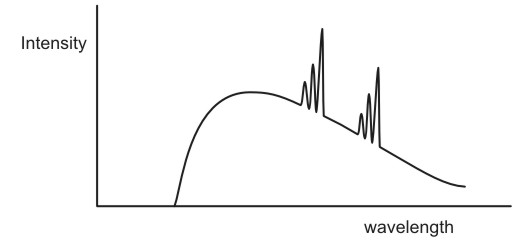
\includegraphics[width = 0.5\textwidth]{./Images/x-ray_spectrum.jpg}
	\caption{Typiskt röntgenspektrum.}
	\label{fig:x-ray_spectrum}
\end{figure}

Röntgenspektrumet är en superposition av ett kontinuerligt spektrum och vissa skarpa toppar. Den kontinuerliga delen kommer direkt från våglängdsspektrumet. De skarpa topparna 
kommer från exitationer av elektroner i metallet. När metallernas elektroner exiteras, skapas det en foton när de hoppar tillbaka till tillståndet med lägre energi, och detta orsakar intensitetstopparna.

\paragraph{de Broglie-våglängd}
Kombinationen
\begin{align*}
	E = h\nu, p = \frac{E}{c}
\end{align*}
för fotoner fick de Broglie att hypotetisera att alla partiklar har en våglängd. Vid att kombinera resultaten ovan, var de Broglies hypotes att denna våglängden ges av
\begin{align*}
	\lambda = \frac{h}{p}.
\end{align*}
Detta kan i stället omformuleras till kinetisk energi vid att använda att
\begin{align*}
	p^{2} &= \frac{1}{c^{2}}E^{2} - m_{0}^{2}c^{2} \\
	      &= \frac{1}{c^{2}}(T^{2} + m_{0}^{2}c^{4} + 2Tm_{0}c^{2}) - m_{0}^{2}c^{2} \\
	      &= \frac{T^{2}}{c^{2}} + 2Tm_{0}, \\
	p     &= \sqrt{2Tm_{0} + \left(\frac{T}{c}\right)^{2}},
\end{align*}
vilket ger
\begin{align*}
	\lambda &= \frac{h}{\sqrt{2Tm_{0} + \left(\frac{T}{c}\right)^{2}}} \\
	        &= \frac{h}{\sqrt{2Tm_{0}}}\frac{1}{\sqrt{1 + \left(\frac{T}{c\sqrt{2Tm_{0}}}\right)^{2}}} \\
	        &= \frac{h}{\sqrt{2Tm_{0}}}\frac{1}{\sqrt{1 + \left(\frac{\sqrt{T}}{c\sqrt{2m_{0}}}\right)^{2}}} \\
	        &= \frac{h}{\sqrt{2Tm_{0}}}\frac{1}{\sqrt{1 + \frac{T}{2m_{0}c^{2}}}}.
\end{align*}

\paragraph{Davidsson-Germers experiment}
I detta experimentet bestrålades en nickelkatod normalt på sin yta med elektroner som accelererades med någon spänning, och reflekterade elektroner detekterades som funktion av vinkel ut från strålen. I detta experimentet uppmättes ett intensitetsmaximum vid en annan vinkel än $0$, och med Braggs formel samsvarar detta maximumet med avståndet mellan atomplan i nickel.

\paragraph{Osäkerhetsprincipen}
de Broglies hypotes säjer att $p$ beror av partikelvågors våglängd i $x$ och $E$ av partikelvågors våglängd i $t$. Vad är en våglängd i $t$? Jo, avståndet i tid mellan två lika punkter på vågen, vilket är perioden, som är direkt kopplad till frekvensen. Detta kombinerad med satser från Fourieranalys implicerar
\begin{align*}
	\Delta p \Delta x \geq \frac{\hbar}{2}, \\
	\Delta E \Delta t \geq \frac{\hbar}{2},
\end{align*}
där vi har infört den reducerade Plancks konstant $\hbar = \frac{h}{2\pi}$.

\paragraph{Vågfunktionen}
Baserad på dessa resultat infördes vågfunktionen $\Psi$. Det postulerades vidare att för alla dynamiska system existerar en vågfunktion som innehåller all information om systemet.
Denna är kontinuerligt deriverbar.

\paragraph{Sannolikhet}
Olika experiment började visa att partiklars position har ett icke-deterministiskt element i sig. Positionen beskrivs av en täthetsfunktion, som postulerades vara $\abs{\Psi}^{2}$.

\paragraph{Schrödingerekvationen}
För ett system av en partikel i en dimension som rör sig i en potential $V$ beskrivs vågfunktionen av
\begin{align*}
	-\frac{\hbar^{2}}{2m}\del{x}{\Psi} + V\Psi = i\hbar\del{t}{\Psi}.
\end{align*}
Detta kan utvidgas för mer allmäna system till
\begin{align*}
	\hat{H}\Psi = i\hbar\del{t}{\Psi},
\end{align*}
där $\hat{H}$ är systemets Hamiltonoperator, som kommer diskuteras sedan.

\paragraph{Bundna tillstånd}
Gör ansatsen $\Psi = \psi(x)\phi(t)$. Då ger Schrödingerekvationen för en enda partikel
\begin{align*}
	-\frac{\hbar^{2}}{2m}\phi\del{x}{\psi} + V\psi\phi = i\hbar\psi\del{t}{\phi}.
\end{align*}
Detta kan separeras till
\begin{align*}
	-\frac{\hbar^{2}}{2m}\frac{\del{x}{\psi}}{\psi} + V = i\hbar\frac{\del{t}{\phi}}{\phi}.
\end{align*}
Om potentialen är tidsoberoende, är vänstersidan bara en funktion av position och högersidan bara en funktion av tid. Därmed måste båda sidor vara lika med en konstant, som vi för tillfället kallar $E$.

Tidsberoendet ger
\begin{align*}
	\del{t}{\phi} &= -i\frac{E}{\hbar}\phi, \\
	\phi          &= Ae^{-i\frac{E}{\hbar}t}.
\end{align*}
Om vi tittar på frekvensen, får vi
\begin{align*}
	\nu = \frac{1}{2\pi}\frac{E}{\hbar} = \frac{E}{h},
\end{align*}
och vi ser att $E$ precis motsvarar partikelvågens energi. Vi noterar vidare att $\abs{\phi}^{2}$ är tidsoberoende, så denna sortens tillstånd ändrar sig inte med tiden.

Positionsberoendet ger nu
\begin{align*}
	-\frac{\hbar^{2}}{2m}\del{x}{\psi} + V\psi = E\psi.
\end{align*}
Alla lösningarna till denna ekvationen är egenfunktioner till operatorn $-\frac{\hbar^{2}}{2m}\del{x}{} + V$ med egenvärde $E$. Utöver detta kan inget säjas utan information om potentialen.

\paragraph{Väntevärde och operatorer}
Eftersom kvantmekaniken handlar om sannolikheter, är även konceptet väntevärde relevant. I kvantmekaniken postulerar vi att det till varje observabel $q$ finns en operator $\hat{q}$, och dens väntevärde ges av
\begin{align*}
	\expval{q} = \integ{}{x}{\cc{\psi}\hat{q}\psi}.
\end{align*}
Exempel på grundläggande operatorer är
\begin{itemize}
	\item positionsoperatorn $\hat{x} = x$.
	\item rörelsemängdsoperatorn $\hat{p} = -i\hbar\del{i}{}$.
	\item kinetisk energi-operatorn $\hat{T} = \frac{1}{2m}\hat{p}^{2}$.
	\item potentialoperatorn $\hat{V} = V$.
	\item Hamiltonoperatorn $\hat{H} = \hat{T} + \hat{V}$.
	\item rörelsemängdsmomentoperatorn $\hat{L}_{i} = \leci{ijk}\hat{r}_{j}\hat{p}_{k}\Leftrightarrow \hat{\vb{L}} = \hat{\vb{r}}\times\hat{\vb{p}}$.
\end{itemize}

\paragraph{Spinn}
Spinn är en ny fysikalisk storhet som dyker upp i kvantmekaniska sammanhang. Den har egenvärden
\begin{align*}
	\abs{S} = \sqrt{s(s + 1)}\hbar
\end{align*}
enligt postulat, där $s$ är ett nytt kvanttal. För elektroner är $s = \frac{1}{2}$.

Alternativt kan man titta på $z$-komponenten av spinnet, med egenvärden
\begin{align*}
	S_{z} = m_{s}\hbar,
\end{align*}
där $m_{s} = 0, \dots, \pm s$ är det spinnmagnetiska kvanttalet.

\paragraph{Fermioner och bosoner}
Alla partiklar kan delas upp i bosoner och fermioner. Om man betraktar den simultana vågfunktionen $\Psi_{1, 2}$ till två lika partiklar, är dessa bosoner om $\Psi_{1, 2} = \Psi_{2, 1}$ och fermioner om $\Psi_{1, 2} = -\Psi_{2, 1}$.

\paragraph{Pauliprincipen}
Fermionerna uppfyller Pauliprincipen, som säger att två ej särskiljbara partiklar ej kan existera i samma individuella kvanttillstånd. Ett typiskt exempel på en fermion är en elektron.

En konsekvens av detta är det faktum att grundämnerna delas upp i periodiska systemet på det sättet de gör.

\paragraph{Magnetiskt moment}
Det magnetiska momentet som skapas av en strömslinga ges av
\begin{align*}
	\vb{\bm{\mu}} = IA\vb{e}_{\text{n}},
\end{align*}
där $I$ är strömmen i slingan, $A$ är ytan som slingan omkransar och $\vb{e}_{\text{n}}$ är en enhetsvektor normalt på slingan enligt högerhandsregeln.

\paragraph{Spinn-bankoppling}
Betrakta en elektron i en cirkulär bana kring en proton. I elektronens system rör protonen sig åt motsatt håll, och dens rörelse orsakar en ström
\begin{align*}
	I &= \frac{e}{T} \\
	  &= \frac{e}{\frac{2\pi r}{v}} \\
	  &= \frac{em_{e}vr}{2\pi m_{e}r^{2}} \\
	  &= \frac{e}{2\pi m_{e}r^{2}}L,
\end{align*}
där $L$ är belopppet av elektronens rörelsemängdsmoment. Det orsakade magnetfältet har flödestäthet
\begin{align*}
	\vb{B} &= -\frac{\mu_{0} I}{2r}\vb{e}_{\text{n}} \\
	       &= -\frac{\mu_{0}}{2r}\frac{e}{2\pi m_{e}r^{2}}\vb{L} \\
	       &= -\frac{\mu_{0}e}{4\pi m_{e}r^{2}}\vb{L}.
\end{align*}
Detta orsakar en potential
\begin{align*}
	V = \vb{\bm{\mu}}_{s}\cdot\vb{B} = -\frac{\mu_{0}e^{2}}{4\pi m_{e}^{2}r^{3}}\vb{S}\cdot\vb{L}.
\end{align*}
Vi ser alltså att den orsakade potentialen beror av elektronens spinn och dens rörelsemängdsmoment. Detta är spinn-bankoppling.

\paragraph{Oändlig lådpotential}
För att få en känsla för vilken sorts fysik som kommer ut av denna teorien, betraktar vi en partikel i en oändlig lådpotential, dvs.
\begin{align*}
	V = 
	\begin{cases}
		0,      &0 < x < a, \\
		\infty, &\text{annars.}
	\end{cases}
\end{align*}
Detta motsvarar en låda med oändligt starka väggar. Rumdelen av Schrödingerekvationen för stationära tillstånd ger inuti lådan
\begin{align*}
	-\frac{\hbar^{2}}{2m}\del{x}{\psi} &= E\psi, \\
	\del{x}{\psi}                      &= -\frac{2mE}{\hbar^{2}}\psi.
\end{align*}
Vi definierar nu
\begin{align*}
	k^{2} = \frac{2mE}{\hbar^{2}}
\end{align*}
och får
\begin{align*}
	\del{x}{\psi} = -k^{2}\psi.
\end{align*}
Detta har lösningar
\begin{align*}
	\psi = Ae^{ikx} + Be^{-ikx}.
\end{align*}

För att få mer information, behövs randvillkor. På grund av vågfunktionens krökningsegenskaper, som framkommer av Schrödingerekvationen, måste vi ha $\psi(0) = \psi(a) = 0$. Första randvillkoret ger
\begin{align*}
	A + B &= 0, \\
	\psi  &= A\sin{kx}.
\end{align*}
Andra randvillkoret ger
\begin{align*}
	ka = n\pi.
\end{align*}
Nu kan energin bestämmas enligt
\begin{align*}
	\frac{n^{2}\pi^{2}}{a^{2}} &= \frac{2mE}{\hbar^{2}}, \\
	E                          &= \frac{\hbar^{2}n^{2}\pi^{2}}{2ma^{2}},
\end{align*}
och vi ser att energin kan bara anta vissa diskreta värden. Vi ser även att grunntilståndets energi är nollskild, som indikerar att ett system som beskrivs av kvantmekaniken alltid kommer ha en viss rörelse.

Slutligen ger normaliseringsvillkoret
\begin{align*}
	\inteval{0}{a}{x}{\abs{B}^{2}\sin^{2}{kx}} = 1.
\end{align*}
Integralen på vänstersidan är
\begin{align*}
	\abs{B}^{2}\inteval{0}{a}{x}{\frac{1 - \cos{2kx}}{2}}.
\end{align*}
Den andra termen ger inget bidrag eftersom den har period $a$, och detta ger
\begin{align*}
	\abs{B}^{2}\frac{a}{2} &= 1, \\
	\abs{B}                &= \sqrt{\frac{2}{a}}.
\end{align*}
Observera att vi endast skriver absolutbeloppet eftersom $B$ kan vara en komplex konstant utan att det ändrar fysiken.

\paragraph{Ändlig lådpotential}
Betrakta en partikel i en ändlig lådpotential, dvs.
\begin{align*}
	V = 
	\begin{cases}
		0,      &0 < x < a, \\
		V_{0},  &\text{annars.}
	\end{cases}
\end{align*}
Detta motsvarar en låda med en viss \"flexibilitet\" i väggarna. Rumdelen av Schrödingerekvationen för stationära tillstånd ger inuti lådan
\begin{align*}
	\del{x}{\psi}                      &= -\frac{2mE}{\hbar^{2}}\psi.
\end{align*}
och
\begin{align*}
	\del{x}{\psi}                      &= -\frac{2m(V_{0} - E)}{\hbar^{2}}\psi.
\end{align*}
Vi definierar som förut
\begin{align*}
	k^{2} = \frac{2mE}{\hbar^{2}}, \alpha^{2} = \frac{2m(V_{0} - E)}{\hbar^{2}}.
\end{align*}
Om $E < V_{0}$ är lösningarna
\begin{align*}
	\psi =
	\begin{cases}
		Ae^{\alpha x},        &x < 0, \\
		Be^{ikx} + Ce^{-ikx}, &0 < x < a, \\
		De^{-\alpha x},       &a < x.
	\end{cases}
\end{align*}
Observera att vissa termer från den matematiska lösningen inte är med, då de skulle ge lösningar som inte är normaliserbara.

%Skriv detta
För att lösa detta, behöver vi de tre villkoren som fås från att $\psi$ är kontinuerligt deriverbar och att $\abs{\psi}^{2}$ är normaliserad.

Vi ser från lösningen att en partikel kan penetrera lite in i en region där dens totala energi är negativ, det så kallade klassiskt förbjudna området. Vi kan även definiera ett penetrationsdjup
\begin{align*}
	\delta = \frac{1}{\alpha} = \frac{\hbar^{2}}{\sqrt{2m(E - V_{0})}}
\end{align*}
som ett mått på hur långt in i den klassiskt förbjudna sonen bundna tillstånd kan penetrera.

\paragraph{Andra potentialer}
Det finns andra intressanta potential att betrakta som kan användas för att beskriva fysikaliska system. Exempel är
\begin{itemize}
	\item det harmoniska potentialet $V = \frac{1}{2}Kx^{2}$, med energiegenvärden $E_{n} = \left(n + \frac{1}{2}\right)\hbar\omega_{0}$, där $\omega_{0} = \sqrt{\frac{K}{m}}$.
\end{itemize}

\paragraph{Bundna system}
Ett bundet system är ett system som är lokaliserad i rummet.

\paragraph{Obundna system}
Ett obundet system är ett system som ej är lokaliserad i rummet.

\paragraph{Ändlig barriär}
Betrakta en partikel i en ändlig lådpotential, dvs.
\begin{align*}
	V = 
	\begin{cases}
		0,      &0 < x, \\
		V_{0},  &\text{annars.}
	\end{cases}
\end{align*}
Detta motsvarar en vägg med en viss \"flexibilitet\".

Man kan definiera en transmissionskoefficient och en reflektionskoefficient lika med sannolikheten för att partiklar transmitteras och reflekteras av barriären.

\paragraph{Tunneling}
Klassiskt kan en partikel inte kryssa en barriär om den har för låg energi. Kvantmekaniskt kan man beräkna en transmissionssannolikhet för tunneling.

Ett enkelt fall som illustrerar tunneling är potential som är konstant lika med $0$ förutom i en region med brädd $a$, där potentialen är $V_{0}$. Schrödingerekvationen ger för detta fallet
\begin{align*}
	T \approx 16\frac{E}{V_{0}}\left(1 - \frac{E}{V_{0}}\right)e^{-2a\sqrt{2m(V_{0} - E)}}, E < V_{0}, a >> \delta.
\end{align*}

Tunneling som fenomen förklarar t.ex. $\alpha$-sönderfall, mikroskopitekniken STM och varför Solen brinner (fusion möjliggörs av att olika atomer kan tunnelera in i varandras kärnor).

\paragraph{Schrödingerekvationen i högre dimensioner}
I högre dimensioner utvidgas Schrödingerekvationen triviellt genom att utvidga definitionen av Hamiltonoperatorn till att verka i alla dimensioner. Även normaliseringen görs över alla dimensioner. Notera att separeringen i tid och rum är exakt likadan.

Ett enkelt exempel är för en partikel, där Hamiltonoperatorn utvidgas till
\begin{align*}
	\hat{H} = -\frac{\hbar^{2}}{2m}\laplacian + V.
\end{align*}

\section{Atomfysik}

\paragraph{Bohrs modell}
För att förklara väteatomens kvantiserade emissionsspektrum, postulerade Bohr att
\begin{itemize}
	\item elektronerna kretsar i stabila banor runt kärnan.
	\item en övergång mellan två banor ger en foton med energi $h\nu = \Delta E$.
	\item elektronens integrerade rörelsemängd längs med banan kring kärnan är en heltalsmultipel av $h$.
\end{itemize}
Om elektronen har konstant rörelsemängd i banan, ger detta
\begin{align*}
	2\pi rp = nh \implies v = \frac{nh}{2\pi m_{e}r},
\end{align*}
där $r$ är banans radius. Accelerationen i radiell riktning ger vidare
\begin{align*}
	\frac{e^{2}}{4\pi\varepsilon_{0}r^{2}} = \frac{m_{e}v^{2}}{r}
\end{align*}
eftersom atomkärnan har samma laddning som elektronen, med motsatt tecken. Enligt Bohrs postulat är de tillåtna banradierna
\begin{align*}
	r_{n} = \frac{\varepsilon_{0}h^{2}}{\pi e^{2}m_{e}}n^{2}.
\end{align*}
Den totala energin ges av
\begin{align*}
	E &= \frac{1}{2}m_{e}v^{2} - \frac{e^{2}}{4\pi\varepsilon_{0}r} \\
	  &= \frac{n^{2}h^{2}}{8\pi^{2}m_{e}r^{2}} - \frac{m_{e}e^{4}}{4\varepsilon_{0}^{2}h^{2}n^{2}} \\
	  &= \frac{m_{e}e^{4}}{8\varepsilon_{0}^{2}h^{2}n^{2}} - \frac{m_{e}e^{4}}{4\varepsilon_{0}^{2}h^{2}n^{2}} \\
	  &= -\frac{m_{e}e^{4}}{8\varepsilon_{0}^{2}h^{2}}\frac{1}{n^{2}}.
\end{align*}
Detta stämde med vätespektrumet.

\paragraph{Väteatomen}
En viktig experimentell kontroll av kvantmekaniken är väteatomens spekter. Bohr lyckades förklara detta med en modell där kvantiseringen av energi introducerades ad hoc, men vi vill nu se om vi får samma spektrumet med hjälp av kvantmekanik.

För att göra detta, vill vi beskriva ett system av en (fix) proton med en elektron i bana runt sig. I sfäriska koordinater med protonen i centrum blir Hamiltonoperatorn
\begin{align*}
	\hat{H} = -\frac{\hbar^{2}}{2m}\left(\frac{1}{r^{2}}\pdv{r}\left(r^{2}\pdv{r}\right) + \frac{1}{r^{2}\sin(\theta)}\pdv{\theta}\left(\sin(\theta)\pdv{\theta}\right) + \frac{1}{r^{2}\sin^{2}(\theta)}\pdv[2]{\phi}\right) - \frac{e^{2}}{4\pi\varepsilon_{0}r}.
\end{align*}
Att ens skriva upp Schrödingerekvationen är extremt jobbigt, så vi försöker i stället att separera den. Detta ger
\begin{align*}
	\frac{\sin^{2}(\theta)}{R}\pdv{r}\left(r^{2}\pdv{R}{r}\right) + \frac{\sin(\theta)}{\Theta}\pdv{\theta}\left(\sin{\theta}\pdv{\Theta}{\theta}\right) + \frac{1}{\Phi}\pdv[2]{\Phi}{\phi} + \frac{2mr^{2}\sin^{2}(\theta)}{\hbar^{2}}\left(E + \frac{e^{2}}{4\pi\varepsilon_{0}r}\right) = 0.
\end{align*}
Vi separerar först bort $\phi$-termen, och setter den lika med en konstant som vi kallar $-m_{l}^{2}$ (som kan vara vad som helst om vi inte exkluderar komplexa tal). Vidare får man
\begin{align*}
	\frac{1}{R}\pdv{r}\left(r^{2}\pdv{R}{r}\right) + \frac{1}{\sin(\theta)\Theta}\pdv{\theta}\left(\sin{\theta}\pdv{\Theta}{\theta}\right) - \frac{m_{l}^{2}}{\sin^{2}(\theta)} + \frac{2mr^{2}}{\hbar^{2}}\left(E + \frac{e^{2}}{4\pi\varepsilon_{0}r}\right) = 0
\end{align*}
Nu kan vi separera igen, med separationskonstant $l(l + 1)$. Vi får alltså tre ekvationer
\begin{align*}
	\frac{1}{\Phi}\pdv[2]{\Phi}{\phi}     &= -m_{l}^{2}, \\
	\frac{1}{R}\pdv{r}\left(r^{2}\pdv{R}{r}\right) + \frac{2mr^{2}}{\hbar^{2}}\left(E + \frac{e^{2}}{4\pi\varepsilon_{0}r}\right) &= l(l + 1), \\
	\frac{1}{\sin(\theta)\Theta}\pdv{\theta}\left(\sin{\theta}\pdv{\Theta}{\theta}\right) - \frac{m_{l}^{2}}{\sin^{2}(\theta)}      &= l(l + 1).
\end{align*}
Vi förenklar till
\begin{align*}
	\pdv[2]{\Phi}{\phi} + m_{l}^{2}\Phi                          &= 0, \\
	\pdv{r}\left(r^{2}\pdv{R}{r}\right) + \frac{2mr^{2}}{\hbar^{2}}\left(E + \frac{e^{2}}{4\pi\varepsilon_{0}r} - l(l + 1)\right)R                        &= 0, \\
	\frac{1}{\sin(\theta)}\pdv{\theta}\left(\sin{\theta}\pdv{\Theta}{\theta}\right) - \left(\frac{m_{l}^{2}}{\sin^{2}(\theta)} + l(l + 1)\right)\Theta &= 0.
\end{align*}
Det här är svårt att lösa, och lösningarna är så speciella att de är namngivna efter olika personer, men randvillkoren kommer att ge
\begin{align*}
	l     &= 0, 1, \dots, n - 1, \\
	m_{l} &= 0, \pm 1, \dots, \pm l.
\end{align*}
$l$ kallas för bankvanttalet och $m_{l}$ kallas för det magnetiska kvanttalet. Det sista kvanttalet $n$ indikerar energin.

Det återstår nu att lösa den radiella ekvationen. Vi gör heller inte det, men de tillåtna energierna är
\begin{align*}
	E = -\frac{m_{e}e^{4}}{8\varepsilon_{0}^{2}h^{2}}\frac{1}{n^{2}} = -\frac{m_{e}e^{4}}{2(4\pi\varepsilon_{0})^{2}\hbar^{2}}\frac{1}{n^{2}}.
\end{align*}
Från detta kan vi definiera Bohrradien
\begin{align*}
	a_{0} = \frac{4\pi\varepsilon_{0}\hbar^{2}}{m_{e}e^{2}}.
\end{align*}

\paragraph{Rörelsemängdsmoment i atomen}
Det visar sig att $Y = \Theta\Phi$ är egentillstånd till båda $\hat{L^{2}}$ och $\vb{L}_{z}$ med egenvärden $\hbar l(l + 1)$ respektiva $\hbar m_{l}$.

\paragraph{Magnetiskt moment i atomen}
Om vi betraktar en elektron i en planär cirkulär bana kring kärnan, ges det magnetiska momentet av
\begin{align*}
	\mu = IA = \frac{e}{\tau}\pi r^{2} = \frac{ev}{2\pi r}\pi r^{2} = \frac{evr}{2} = \frac{e}{2m_{e}}\abs{\vb{L}}.
\end{align*}
Från detta får vi en vektor
\begin{align*}
	\vb{mu} = -\frac{e}{2m_{e}}\vb{L},
\end{align*}
och speciellt
\begin{align*}
	\mu_{z} = -\frac{e}{2m_{e}}L_{z} = -\frac{e\hbar}{2m_{e}}m_{l} = -\mu_{\text{B}}m_{l},
\end{align*}
där vi har definierat Bohrmagnetonen
\begin{align*}
	\mu_{\text{B}} = \frac{e\hbar}{2m_{e}}.
\end{align*}

Om vi nu applicerar ett externt magnetiskt fält i $z$-riktningen, ger detta upphov till en potential
\begin{align*}
	U = -\vb{\mu}\times\vb{B} = \mu_{\text{B}}m_{l}B.
\end{align*}

Även spinnet ger upphov till ett magnetiskt moment
\begin{align*}
	\vb{\mu}_{S} = -g{S}\frac{e}{2m_{e}}\vb{S},
\end{align*}
där $g_{S}$ är det gyromagnetiska förhållandet som (nästan) alltid är lika med $2$.

\paragraph{Zeeman-effekten}
När en atom är i ett externt magnetiskt fält, splittas atomspektrumet därför att olika rörelsemängdsmoment har olika energier på grund av den uppkomna potentialen.

\paragraph{Stern-Gerlachs experiment}
Potentialen som uppkommer av ett externt magnetiskt fält ger upphov till en kraft
\begin{align*}
	\vb{F} &= -\grad{-\vb{\mu}\times\vb{B}}, \\
	F_{z}  &= \mu_{z}\del{z}{B}\vb{e}_{z} = -\frac{e\hbar}{2m_{e}}m_{l}\del{z}{B}\vb{e}_{z}.
\end{align*}

Det gjordes därför ett experiment där elektroner sköts genom ett magnetfält som ökade i styrka uppåt och fångades upp av en skärm. Baserad på resultaten från rörelsemängdsmomentet, skulle elektronerna fångas upp i ett udda antal olika punkter, men detta var inte fallet. Specifikt, då de förväntade att alla elektroner skulle hamna i samma punkt ($l = 0$), hamnade de i stället i två olika punkter. Detta måste uppkomma från spinnet.

\paragraph{Masstal}
En atomkärna har $Z$ protoner, $N$ neutroner och masstal $A = N + Z$. Olika isotoper betecknas då som $^{A}_{Z}\text{X}_{N}$, eller bara $^{A}\text{X}$.

\paragraph{Kärnans täthet}
Man har (möjligtvis experimentellt) att kärnans radie är proportionell mot $A^{\frac{1}{3}}$, och detta ger
\begin{align*}
	\rho = \frac{V}{m} \propto \frac{A}{A} = 1,
\end{align*}
och kärnans täthet beror ej av masstalet.

\paragraph{Experiment som avslöjade atomkärnan}
Under tidiga $1900$-talet trodde man att atomen var kontinuerlig, med en positivt laddad smet som omkransade negativt ladda elektroner. I $1911$ kom Rutherford på ett experiment som gjordes av Geiger och Marsden, där en stark $\alpha$-källa bombarderade en guldfilm. Enligt den dominerande modellen skulle $\alpha$-partiklerna gå direkt igenom och spridas minimalt. Däremot spriddes vissa $\alpha$-partiklar mycket, vilket implicerade att i atomens centrum fantes en tung kärna där det mesta av massan var koncentrerad. Vidare bytte han ut guldfilmen med en aluminiumsfilm. Eftersom det är färre protoner i aluminiums kärna, är det svagare repulsion mellan atomkärnan och $\alpha$-partikeln, vilket gjorde att de i detta experimentet lyckades träffa atomkärnan.

\section{Kärnfysik}

\paragraph{Fundamentala begrepp}
En atomkärna har ett visst antal av protoner och neutroner. Antal protoner $Z$ kallas protontalet, antal neutroner $N$ kallas neutrontalet och $A = N + Z$ kallas nukleontalet.

\paragraph{Atomkärnans storlek}
Experimentella resultat har gett
\begin{align*}
	R = R_{0}A^{\frac{1}{3}},
\end{align*}
där $R_{0}$ är en konstant. Resultatet blir att volymen är linjär i nukleontalet, vilket kan tolkas som att kärnans nukleontäthet (och därmed även masstäthet) ej beror av nukleontalet.

\paragraph{Bindningsenergi och Weiszäckers formel}
Bindningsenergin för olika ämnen varierar starkt. Ett försök på att beskriva detta kom från Weiszäcker och Bethe. De betraktade atomkärnan som en laddad vätskedroppe. Efter att introducera lite extratermer för att få formeln att passa med trender från experiment, kom de fram till
\begin{align*}
	E = a_{V}A - a_{S}A^{\frac{2}{3}} - a_{C}Z(Z - 1)A^{-\frac{1}{3}} - a_{\text{sym}}\frac{(A - 2Z)^{2}}{A} + \delta,
\end{align*}
där $\delta$ är $a_{P}A^{-\frac{3}{4}}$ om både $Z$ och $N$ är jämna, $-a_{P}A^{-\frac{3}{4}}$ om både $Z$ och $N$ är udda och $0$ om $A$ är udda.

Första termen är linjär i $A$, precis som kärnans volym, och kallas ofta volymtermen. Den har sitt ursprung i starka kärnkraften. Andra termen kommer från effekter på kärnans yta. Tredje termen kommer från repulsion mellan protoner i kärnan. Tredje termen kommer från att nukleonerna är fermioner, och därför ökar kärnans energi omdet finns många lika nukleoner som behöver olika tillstånd. Den sista termen kommer från spinn-bankoppling i kärnan, och beror på att energin blir lägre om det finns lika många partiklar med spinn upp och ned.

Jämförelser med experimentella resultat visar att det stämmer ganska väl, förutom för vissa värden på $N$ och $Z$, där kärnan är mycket mer stabil än vad denna formeln skulle förutspå. Dessa speciella värden kallas för magiska tal.

\paragraph{Skalmodell för atomkärnan}
Om man i stället betrakter nukleonerna som partiklar i en sfärisk låda med oändligt starka väggar, får man skallösningar för energierna. Vid att även introducera spinn-bankoppling lyckades denna enkla modellen återskapa magiska tal som stämde med experiment. För sitt arbet med detta fick Maria Goeppert-Mayer, Johannes Jensen och Eugene Wigner Nobelpriset i 1963.

\paragraph{Radiokativitet}
Radioaktivitet är ett begrepp för processer där atomkärnan förändras. För att en radioaktiv process skall ske (spontant), måste
\begin{itemize}
	\item processen ge från sig energi.
	\item konserveringslagarna för laddning, rörelsemängd, rörelsemängdsmoment, nukleontalet (inte i allmänna kärnprocesser), leptontalet och universums totala energi vara uppfyllda.
\end{itemize}

\paragraph{Aktivitet}
Den radioaktiva aktiviteten definieras som
\begin{align*}
	A = -\dv{N}{t}
\end{align*}
där $N$ är antal radioaktiva partiklar i systemet. Experimentellt avtar exponentiellt med tiden, vilket enkelt kan förklaras om aktiviteten är proportionell med antal radioaktiva partiklar.

\paragraph{Halveringstid}
Om man gör ansatsen $A = \lambda N$ får man $A\propto e^{-\lambda t}$. Halveringstiden $t_{\frac{1}{2}}$ definieras som tiden det tar för aktiviteten (eller, ekvivalent, antal radioaktiva partiklar) att halveras relativt ursprungsaktiviteten. Från detta relateras konstanten till halveringstiden med
\begin{align*}
	\lambda = \frac{\ln{2}}{t_{\frac{1}{2}}}.
\end{align*}

\paragraph{$Q$-värde}
$Q$-värdet för en radioaktiv process är den totala ändringen i energi för processen.

\paragraph{$\alpha$-sönderfall}
I $\alpha$-sönderfall ger kärnan från sig en He-kärna med $2$ protoner och $2$ neutroner. Energispektrumet för denna processen är diskret.

Man kan räkna fram att $\alpha$-partikelns energi ges av
\begin{align*}
	E_{\alpha} = \frac{Q}{1 + \frac{m_{\alpha}}{m_{\text{ny}}}},
\end{align*}
där $m_{\text{ny}}$ är den nya kärnans massa. Energispektrumet är alltså diskret.

\paragraph{$\beta^{-}$-sönderfall}
I $\beta^{-}$-sönderfall omdannas en neutron till en proton, och det skapas i processen en elektron och en elektron-antineutrino med symbolen $\bar{\nu}_{e}$. $\bar{\nu}_{e}$ är i princip masslös. Eftersom två partiklar skapas, är energifördelningen för $\beta^{-}$-partikeln (elektronen) kontinuerlig för energier upp till processens $Q$-värde.

Reaktionens $Q$-värde ges av
\begin{align*}
	Q_{\beta^{-}} &= (m_{N, Z} - m_{N - 1, Z + 1} - m_{e^{-}})c^{2} \\
	              &= (M_{N, Z} - M_{N - 1, Z + 1})c^{2},
\end{align*}
där $m$ refererar till kärnmassan och $M$ den totala atommassan (massan av kärnan och elektronerna). Villkoret för att reaktionen skall ske är
\begin{align*}
	M_{N, Z} > M_{N - 1, Z + 1}.
\end{align*}

\paragraph{$\beta^{+}$-sönderfall}
I $\beta^{+}$-sönderfall omdannas en proton till en neutron, och det skapas i processen en positron, med symbol $e^{+}$ och en elektronneutrino med symbolen $\nu_{e}$. Eftersom två partiklar skapas, är energifördelningen för $\beta^{+}$-partikeln (positronen) kontinuerlig för energier upp till processens $Q$-värde.

Reaktionens $Q$-värde ges av
\begin{align*}
	Q_{\beta^{-}} = (M_{N, Z} - M_{N + 1, Z - 1} - 2m_{e})c^{2},
\end{align*}
där vi nu ser att den nya atomen har plats till en mindre elektron och att vi har skapat en positron (som har massan $m_{e}$). Villkoret för att reaktionen skall ske är
\begin{align*}
	M_{N, Z} > M_{N + 1, Z - 1} + 2m_{e}.
\end{align*}

\paragraph{$\gamma$-strålning}
Atomkärnans energinivåer är även kvantiserade. När kärnan hoppar ned i sina energinivåer, skickas det ut en foton. Gammastrålning kan förekomma efter andra radioaktiva processer, när atomkärnan efter processen är kvar i ett högt energinivå och hoppar ned. Sådana processer har ofta kort halveringstid.

\paragraph{Elektroninfångning}
I elektroninfångning fångas en elektron in i atomkärnan, och bildar till sammans med protonen en neutron. Från detta skickas även ut en $\nu_{e}$.

Under processen dyker även upp ett ookkuperat elektrontillstånd i en av de innersta orbitalerna. När en elektron hoppar ned till detta tillståndet, skickas karakteristisk röntgenstrålning ut. Denna strålningen har ett diskret energispektrum.

\paragraph{Inre konversion}
I stället för att göra sig av med energi genom $\gamma$-sönderfall, kan kärnan ge energin till en elektron som exiteras. Denna processen har ett diskret energispektrum. På samma sättet som med elektroninfångning följer karakteristisk strålning ut efter detta.

\paragraph{Spontan fission}
Vissa atomkärnor kan spontant deformeras och dela sig upp i två delar samt några neutroner. Det mesta av energin för sådana processer går till de två fissionsprodukterna. 

\section{Molekylfysik}

\paragraph{Molekyler}
Molekyler är enheter som består av ett antal atomer.

\paragraph{Frihetsgrader}
Jämförd med atomer, kan molekyler både vibrera och rotera.

\paragraph{Modellpotential}
Om vi betraktar en elektron som är bunden av två atomer, försöker vi beskriva den med en potential på formen
\begin{align*}
	V(r) = -\frac{A}{r^{n}} + \frac{B}{r^{m}}
\end{align*}
i en dimension. De involverade konstanterna kan anpassas till experiment, men för att elektronen inte skall dras in mot en atomkärna, måste $m > n$.

Derivatan av detta ges av
\begin{align*}
	\dv{V}{r} = \frac{nA}{r^{n + 1}} - \frac{mB}{r^{m + 1}},
\end{align*}
och potentialens minimum ges av
\begin{align*}
	\frac{nA}{r^{n + 1}} - \frac{mB}{r^{m + 1}} &= 0, \\
	nA                                          &= \frac{mB}{r^{m - n}} \\
	r                                           &= \left(\frac{mb}{nA}\right)^{\frac{1}{m - n}}.
\end{align*}

\paragraph{Jonbindning}
Om man har två atomer, där den ena har en löst bunden elektron och den andra har ett ookkuperat tillstånd i sitt ytterste fyllda skal, kan den löst bundna elektronen övergå från ena atomen till den andra. Detta resulterar i en nettoladdning på varje atom, vilket skapar en attraherande kraft, även kallad en jonbindning. Jonkristaller som bildas av fler atomer förklaras analogt.

Utbytet av elektroner i sig själv är inte gynnsamt utan det som gör att salter bildas spontant är kombinationen av elektronutbyte och Coulombvexelvärkan.

Vid små avstånd mellan atomen får man repulsiva krafter både från Paulirepulsion mellan elektronerna och Coulombrepulsion mellan kärnorna (effekten av dessa beror på avståndet mellan atomerna), varför modellpotentialen ovan är en bra beskrivning av interaktionen mellan atomerna.

\paragraph{Kovalent bindning}
Kovalent bindning uppstår när två atomer delar på sina elektroner.

Som ett exempel, betrakta två lika atomer $A$ och $B$. En ungefärlig lösning till Schrödingerekvationen för en elektron är $\Psi = a\Psi_{A} + b\Psi_{B}$. Av symmetriskäl är $a = \pm b$. Detta ger upphov till en symmetrisk och en antisymmetrisk lösning.

I enkla fall som väte kan detta lösas numeriskt. Då kan man jämföra energierna för små och stora avstånd mellan atomerna. Det man får är att den symmetriska lösningen har lägre energi än den antisymmetriska. Den symmetriska lösningen har hög sannolikhetstäthet mellan atomerna, medan den antisymmetriska lösningen har låg täthet mellan atomerna. Därmed kan detta tolkas som att den symmetriska lösningen ger ett elektronmoln mellan atomerna som attraherar båda, medan den antisymmetriska lösningen ger ett molm som omringar två atomer som repelleras.

\paragraph{Rotation}
Till skillnad från atomer kan molekyler rotera. Det är detta vi vill beskriva.

Betrakta en stel kropp av två punktmassor som roterar i planet i deras masscentrumssystem. Detta är ekvivalent med en stel kropp med massa $\mu = \frac{m_{1}m_{2}}{m_{1} + m_{2}}$ som roterar kring kroppens masscentrum med ortsvektor $R = r_{1} + r_{2}$.

Varför funkar detta? Det korta svaret är att det första systemet har rörelsemängdsmoment
\begin{align*}
	L = m_{1}\omega r_{1}^{2} + m_{2}\omega r_{2}^{2}
\end{align*}
normalt på rörelsesplanet. Det är klart att eftersom kroppen roterar kring sitt masscentrum är $r_{1} = -\frac{m_{2}}{m_{1}}r_{2}$, vilket ger
\begin{align*}
	L &= \frac{m_{2}^{2}}{m_{1}}\omega r_{2}^{2} + m_{2}\omega r_{2}^{2} \\
	  &= \frac{m_{2}^{2} + m_{1}m_{2}}{m_{1}}\omega r_{2}^{2}.
\end{align*}
Om man inför det totala avståndet $R$ mellan partiklerna, får man vidare $-r_{1} + r_{2} = \frac{m_{2} + m_{1}}{m_{1}}r_{2} = R$ och $r_{2} = \frac{m_{1}}{m_{2} + m_{1}}R$, vilket ger
\begin{align*}
	L &= \frac{m_{1}m_{2}}{m_{2} + m_{1}}\omega R^{2},
\end{align*}
vilket skulle visas.

Kroppens rörelsemängdsmoment ges av $L = \mu v\times R$ och dens tröghetsmoment med avseende på masscentrum ges av $I = \mu R^{2}$. Då kan rotationsenergin skrivas som
\begin{align*}
	E = \frac{L^{2}}{2I}.
\end{align*}
Detta systemet är sfäriskt symmetriskt, varför rörelsemängdsmomentet är kvantiserad som $L^{2} = \hbar^{2}j(j + 1), j = 0, 1, \dots$, där $j$ är kvanttalet som beskrivar rotationen. Då ges rotationsenergin av
\begin{align*}
	E = \frac{\hbar^{2}j(j + 1)}{2I}.
\end{align*}

\paragraph{Vibrationer}
Bindningarna i molekyler kan vibrera, och det är detta vi vill beskriva.

För att beskriva vibrationerna i en bindning, ansätter vi att atomerna i bindningen interagerar med Morse-potentialen
\begin{align*}
	V(r) = V_{0}\left(1 - e^{-\beta(r - r_{0})}\right)^{2}.
\end{align*}
Nära $r_{0}$ kan detta approximeras som en harmonisk oscillator med styrka $k = 2V_{0}\beta^{2}$. Detta ger upphov till energinivåer
\begin{align*}
	E = (v + \frac{1}{2})\hbar\omega_{0}, v = 0, 1, \dots
\end{align*}
där $\omega_{0} = \sqrt{\frac{k}{\mu}}$.

\paragraph{Energiövergånger}
Om en molekyl skall ändra sitt tillstånd, kan detta endast hända under förutsättningen $\Delta j = \pm 1$ för att bevara rörelsemängdsmomentet och $\Delta v = \pm 1$ eftersom molekylen interagerar bäst med fotoner under denna förutsättning (för låga energier). Detta ger till exempel upphov till rotations-vibrationsspektra.

\section{Fasta tillståndets fysik}

\paragraph{Kristaller}
Kristaller är en underkategori av fasta ämnen där atomerna i ämnet har en viss ordning. Mer specifikt är atomerna ordnade i ett mönster som upprepas perfekt i hela kristallen.

De flesta reella kristallinska ämnen är byggda upp av många små kristaller, där dessa gärna har olika orienteringar relativt varandra.

\paragraph{Bindning i kristaller}
Kristaller är oftast bundna av jonbindningar, kovalenta bindningar eller metallbindningar. Och vad är nu metallbindinigar?

\paragraph{Metallbindningar}
Atomerna i en kristall kan bindas av metallbindningar. Detta uppstår när atomerna i kristallen ger från sig sina elektroner. Elektronerna bildar en gas, medan de positiva metallatomerna hålls ihop av en balans mellan attraktion till elektrongasen och repulsion mellan andra atomer.

\paragraph{Materialers elektriska egenskaper}
Alla materialer kan delas i
\begin{itemize}
	\item isolatorer, som har väldigt hög resistivitet.
	\item ledare, som har väldigt låg resistivitet.
	\item halvledare, som har egenskaper någon stans mittemellan.
\end{itemize}

\paragraph{Bandstruktur}
Energinivåerna för en enda atom är kvantiserade, men i en kristalll kan elektronen leva överallt runt de olika atomerna. De tillåtna energinivåerna för elektronerna i en kristall konvergerar då mot intervall med tillåtna energier, så kallade energiband. Hur dessa banden ser ut för ett material kallas för materialets bandstruktur, och är närt kopplad till de elektriska egenskaperna.

\paragraph{Valensband och ledningsband}
Valensbandet är det bandet med högst energi som har elektroner i sig. Ledningsbandet är det bandet med lägst energi som har ookkuperade elektrontillstånd. Gapet mellan dessa kallas för bandgapet.

\paragraph{Ledares bandstruktur}
I en ledare krävs relativt låg energi för att exitera elektronerna med högst energi så att de kan röra på sig i kristallen. I termer av bandstruktur kan man säja att valensbandet och ledningsbandet är det samma, eller att bandgapet är litet. Eftersom denna processen kräver lite energi, är den spontan, och därmed ledar ledare elektricitet väl.

\paragraph{Isolatorers bandstruktur}
I en isolator är bandgapet stort, och det är svårt för elektroner att exiteras och börja röra på sig. Därmed ledar de elektricitet dåligt.

\paragraph{Halvledares bandstruktur}
Halvledare har ett bandgap som är någon stans imellan, vilket ger de vissa mer exotiska egenskaper.

\paragraph{Fyllning av band}
Elektroner fyller tillstånd i band med en given energi med en sannolikhet enligt Fermi-Dirac-fördelningen
\begin{align*}
	f(E) = \frac{1}{1 + e^{\frac{E - \mu}{kT}}}.
\end{align*}

\paragraph{Dopning av halvledare}
Dopning av en halvledare är att tillsätta olika andra ämnen till den. Detta gör att man kan ändra dens elektriska egenskaper, antingen vid att tillföra ookkuperade elektrontillstånd nära valensbandet eller fyllda elektrontillstånd nära ledningsbandet.

\paragraph{Supraledare}
Vissa materialer förlorar all sin resistivitet när de kyls ned till väldigt låga temperaturer. Dessa kalles supraledare.

\section{Partikelfysik}

Partikelfysik är läran om universums minsta beståndsdelar.

De första partiklarna vi upptäckte var de som bygger upp atomen. Efter det upptäcktes partiklar från kosmisk strålning. För att upptäcka nya partiklar konstruerade vi partikelacceleratorer för att försöka bilda nya partiklar.

\paragraph{Elementarpartiklar}
En elementarpartikel är en odelbar partikel. Vi tror att alla elementarpartiklar kan delas upp i kvarkar och leptoner.

\paragraph{Kvarkar}
Det finns $6$ kvarkar:
\begin{table}[!ht]
	\begin{tabular}{| c | c | c |}
		\hline
		                    & $q = \frac{2}{3}$ & $q = -\frac{1}{3}$ \\
		\hline
		Spinn $\frac{1}{2}$ & Upp, $u$          & Ned, $n$ \\
		\hline
		                    & Charm, $c$        & Konstig, $s$ \\
		\hline
		                    & Topp, $t$         & Botten, $b$ \\
		\hline
	\end{tabular}
\end{table}

Protonen bildas som $uud$, och neutronen som $udd$. Man kan undra på om de lika kvarkerna är i samma kvanttillstånd. Detta är inte fallet på grund av färgladdning.

\paragraph{Leptoner}
Det finns även $6$ leptoner:
\begin{itemize}
	\item elektronen.
	\item muonen.
	\item taupartikeln.
	\item neutrioner motsvarande varje partikel.
\end{itemize}
Alla dessa är fermioner med spinn $\frac{1}{2}$.

\paragraph{Antipartiklar}
Till varje elementarpartikel tillhör även en antipartikel med motsatta kvanttal.

\paragraph{Utbytespartiklar}
I partikelfysiken förmedlas alla krafter med hjälp av så kallade utbytespartiklar. Det finns:
\begin{itemize}
	\item gluonen, som förmedlar stark växelverkan. Den är masslös och har färgladdning.
	\item fotonen, som förmedlar elektromagnetisk växelverkan. Den är masslös och har ej färgladdning.
	\item $Z$-bosonen.
	\item $W$-bosonen.
\end{itemize}
Alla har spinn $1$.

\paragraph{Bevarandelagar}
De viktigaste bevarandelagarna som spelar roll i partikelfysiken är bevarandet av
\begin{itemize}
	\item energi.
	\item rörelsemängd.
	\item laddning.
	\item antal kvarkar.
	\item alla leptontal.
	\item baryontalet.
	\item kvarksmak, förutom i reaktioner med $W$.
\end{itemize}

\paragraph{Invarianta massan}
Betrakta ett sönderfall där en partikel sönderfallar till vissa andra partiklar. Speciell relativitet ger
\begin{align*}
	E^{2} = p^{2}c^{2} + m^{2}c^{4},
\end{align*}
vilket kan lösas för massan för att ge
\begin{align*}
	m^{2}c^{4} = E^{2} - p^{2}c^{2}.
\end{align*}
Eftersom energin och rörelsemängden bevaras, kan detta skrivas som
\begin{align*}
	m^{2}c^{4} = \left(\sum E_{i}\right)^{2} - \left(\sum p_{i}\right)^{2}c^{2},
\end{align*}
där det summeras över energierna och rörelsemängderna till sönderfallsprodukten. Detta ger upphov till begreppet invariant massa.

\end{document}
